\documentclass{article}
\usepackage[utf8]{inputenc}

\usepackage[margin=1in]{geometry}
\usepackage{amsmath,amsthm,amssymb}
\usepackage[margin=1in]{geometry}
\usepackage{amsmath,amsthm,amssymb}
\usepackage[spanish]{babel} %Castellanización
\usepackage[T1]{fontenc} %escribe lo del teclado
\usepackage[utf8]{inputenc} %Reconoce algunos símbolos
\usepackage{lmodern} %optimiza algunas fuentes
\usepackage{graphicx}
\usepackage{relsize}
\graphicspath{ {images/} }
\usepackage{hyperref} % Uso de links


\title{Resumen T-K$^2$raster}
\author{}
\date{}

\begin{document}

\maketitle

\section*{Related work}
Es importante que primero contextualicemos hablando acerca de las estructuras e
ideas precursoras al T-k2raster.\\
El objetivo principal es la representación de raster time series como una
estructura de datos compacta, ya que esta nos perimte trabajar de forma eficiente,
permitiendo consultas sobre los datos sin la necesidad de descomprimir estos.\\
Más aún queremos aprovechar la localidad de los datos, es decir, aprovechar las
regularidades temporales que existen entre instantes de tiempo cercanos.

\subsection*{Rank y select en bitmaps}
\begin{itemize}
  \item Definimos las operaciones de rank y select para bitmap, las cuales serán
    usadas durante todo este trabajo.
  \item Considere un bitmap $B[0 \ldots n-1]$, que guarda una secuencia de $n$
    bits.
  \item $rank_a(B, i) $: cuenta las apariciones del bit $a$ en $B[0 \ldots i]$.
  \item $select_a(B,i)$: localiza la posición de la $i$-ésima ocurrencia de
    $a$ en $B$.
\end{itemize}

\subsection*{Quadtree}
\begin{itemize}
  \item Árbol donde cada nodo, excepto las hojas, tienen cuatro hijos.
  \item Tamaño potencia de 2.
  \item Representada por una matriz la cual se subdivide en cuatro cuadrados
    (quadboxes) recursivamente hasta cumplir alguna condición de termino dada.
  \item A un nodo se le asigna un label de ''1'' si este contiene hijos con
    label ''1''. Se le asigna un 0 en caso contrario.
  \item Los nodos con label 0 no se siguen dividiendo, mientras los que tienen
    label 1 sigue hasta encontrar un quadbox vacío o las celdas individuales del
    raster.
  \begin{figure}[h]
    \centering
    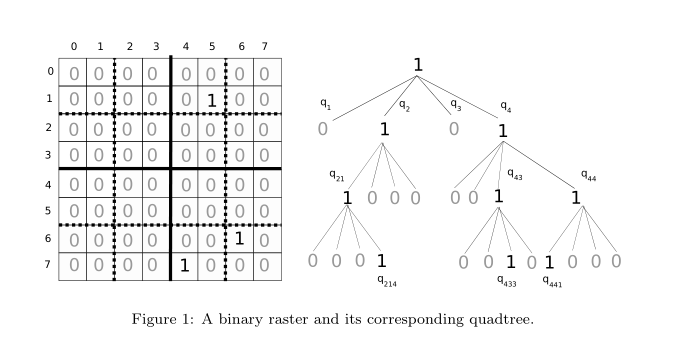
\includegraphics[width=0.57\textwidth]{../images/quad.png}
  \end{figure}
\end{itemize}

\subsubsection*{K$^2$tree}
\begin{itemize}
  \item Corresponde a un region quadtree (para $k = 2$) donde los nodos del árbol se almacenan
    siguiendo el orden de una búsqueda en anchura.
  \item Por practicidad los nodos se almacenan en dos arreglos, $L$ formado por
    los bits del último nivel (leafs), y $T$ donde se almacena el resto de nodos.
  \item Dada una posición $p$ en $T$ con valor 1, podemos obtener la posición
    donde los $k^2$ hijos de $p$ comienzan de la siguiente forma: \[
      p_{hijos} = rank_1(T, p) \cdot k^2
    \]
  \item En el caso que $p_{hijos}$ corresponda a hojas, ($p_{hijos} > |T|$)
    podemos obtener su posición como\\ $L[p_{hijos} - |T|]$.
  \item La consulta $rank$ se puede efectuar en tiempo constante, agregando una
    \emph{estructura de rank} sobre $T$, la cual usa un espacio sublinear.
\end{itemize}

\subsubsection*{K$^3$tree}
\begin{itemize}
  \item Es la extensión del k$^2$tree añadiendo una dimensión más.
  \item Para $k = 2$ se representa por un octree.
  \item Se puede navegar eficientemente utilizando los mismos métodos del
    k$^2 $tree, pero extendido a tres dimensiones.
\begin{figure}[h]
  \centering
  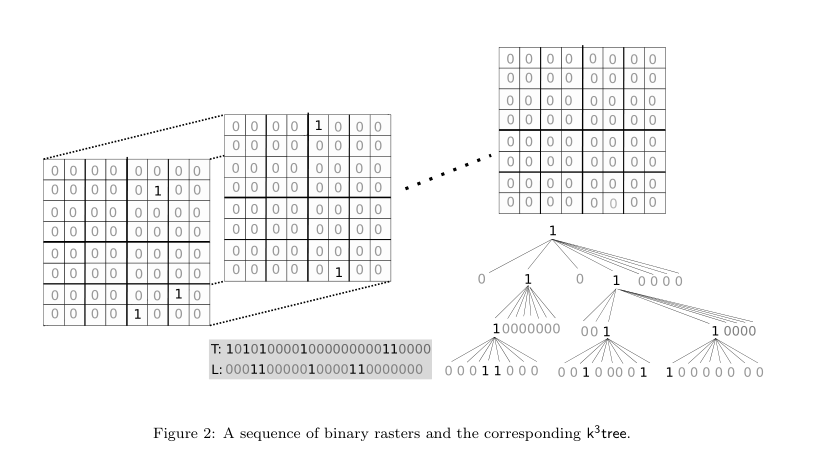
\includegraphics[width=0.8\textwidth]{../images/k3tree.png}
\end{figure}
\end{itemize}


\subsection*{Compact representation of rasters}

\subsubsection*{k$^2$raster}
\begin{itemize}
  \item Además de almacenar matrices binarias como lo hace el k$^2$tree, puede
    almacenar matrices de enteros.
  \item Divide el espacio de manera similar al k$^2$tree, pero los nodos
    del árbol almacenan los valores máximos y mínimos de su quadtree
    correspondiente.
  \item La subdivisión termina cuando los valores max y min son iguales, o cuando
    se llega la las celdas del raster.
  \item Utiliza un arreglo de bits para representar la topología del árbol,
    y codificación diferencial para los enteros.
  \begin{figure}[h]
    \centering
    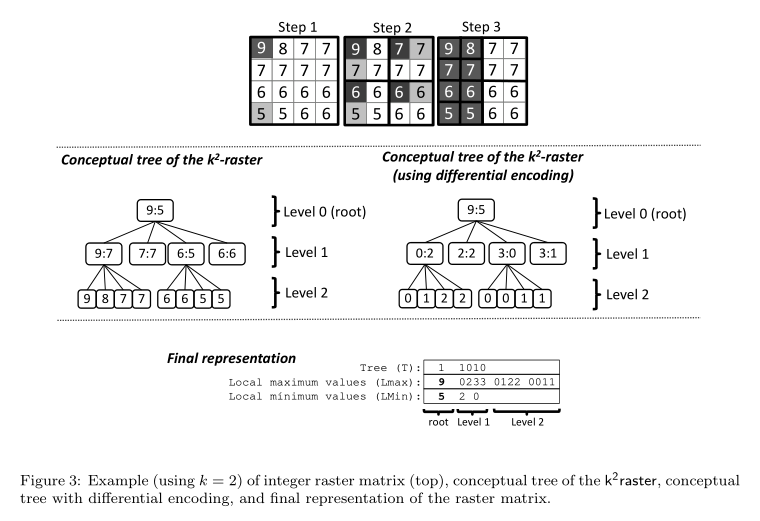
\includegraphics[width=0.8\textwidth]{../images/k2raster.png}
  \end{figure}
  \item Los valores max y min de cada nodo son codificados respecto a la
    diferencia que existe entre el max y min del nodo padre. Las hojas por
    defecto se comparan con el máximo.
   \item Estas diferencias son almacenadas en dos secuencias,
     \emph{Lmax} y \emph{Lmin}, siguiendo una búsqueda en anchura a través del
     árbol conceptual.
\end{itemize}

\subsubsection*{3D2D-mapping}
\begin{itemize}
  \item Método para tranformar una matriz que representa un raster, en una matriz
    binaria la cual se almacena en un k$^2$tree para obtener compresión y
    consultas rápidas directamente en el.
  \item La transformación se basa en el \emph{Morton order}, también conocido
    como \emph{Z-order}, el cual cuenta con una buena preservación de la
    localidad espacial.
  \item Mapea desde un espacio multidimensional a un espacio unidimensional.
    \begin{figure}[h]
      \centering
      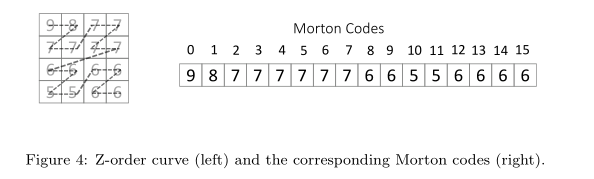
\includegraphics[width=0.8\textwidth]{../images/morton.png}
    \end{figure}
  \item Sea el vector creado $V$, se construye la matriz binaria $BM$ de la
    siguiente forma: \\
    \[
      \text{La celda } BM[x][y] \text{ se setea en 1 si } V[x] = y
      \text{, de otra forma, se almacena un 0}
    .\]
    \begin{figure}[h]
      \centering
      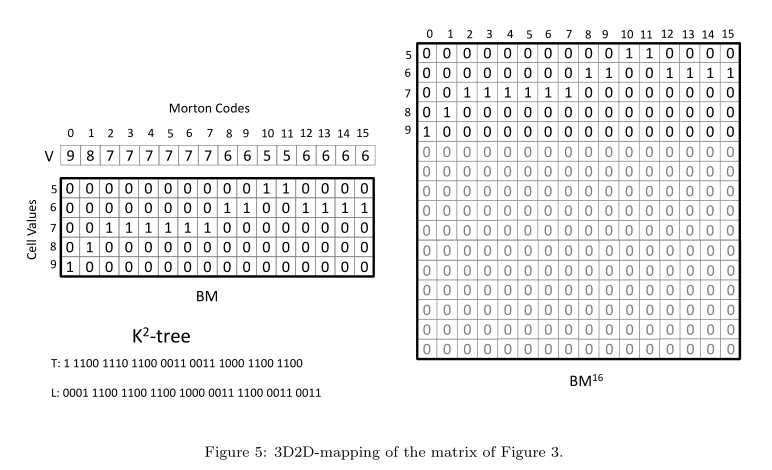
\includegraphics[width=0.8\textwidth]{../images/3d2d.png}
    \end{figure}
  \item El k$^2$tree requiere almacenar matrices de tamaño $n \times n$ donde
    $n$ es una potencia de 2.
  \item Si $BM$ es de tamaño $r \times c$, se extiende a tamaño $n \times n$ con
    bits 0 en las celdas creadas, siendo $n$ la potencia de 2 más pequeña
    que sea mayor o igual a $r$ y $s$. Esta matriz es llamada $BM^n$.
  \item Finalmente es representado el k$^2$tree el cual es capaz de almacenar
    grandes áreas llenas de 0-bits, y como se puede apreciar, utiliza mucho menos
    espacio que $BM$ y $BM^2$.
  \item Ahora, se pueden obtener los valores de una celda o ventana de la matriz
    utilizando las consultas para k$^2$tree.
\end{itemize}

\subsection*{Compact representation of raster times series}
\subsubsection*{4D3D-mapping}
\begin{itemize}
  \item Basado en 3D2D-mapping.
  \item Se utiliza el mapping para obtener una matriz binaria por cada raster
    representando un instante de tiempo.
  \item Las matrices binarias se extienden con bits 0 hasta obtener un cubo 3D
    perfecto de tamaño $m \times m \times m$, siendo $m$ la menor potencia de 2
    mayor que $r \times s \times \tau$, donde $\tau$ es la cantidad de instantes
    de tiempo.
  \item El cubo binario resultante es almacenado utilizando un $k^3$tree. El
    cual provee almacenamiento comprimido y consultas rápidas directamente en el.
  \item Dado los raster originales $M = (M_1,M_2,\ldots,M_\tau)$, se les aplica
    el 3D2D mapping a cada $M_i$, obteniendo así $(BM_1,BM_2,\ldots,BM_\tau)$,
    matrices binarias. Recordar que todas las matrices tienen tamaño $r\times c$.
  \item Definimos a $BM^m_i$ como:
    \begin{itemize}
      \item Para $1 \le i \le \tau$, $BM_i$ se extiende con bits 0 hasta obtener
        una matriz de $m \times m$.
      \item Para $\tau + 1 \le i \le m$, se agrega una matriz de tamaño
        $m \times m$ llena de bits 0.
    \end{itemize}
  \item Finalmente el 4D3D-mapping se obtiene al guardar $(BM_1^m,BM_2^m,\ldots,
    BM_m^m)$ en un $k^3$tree de tamaño $m \times m \times m$, llamado $BC$
    (binary cube).
      \centering
      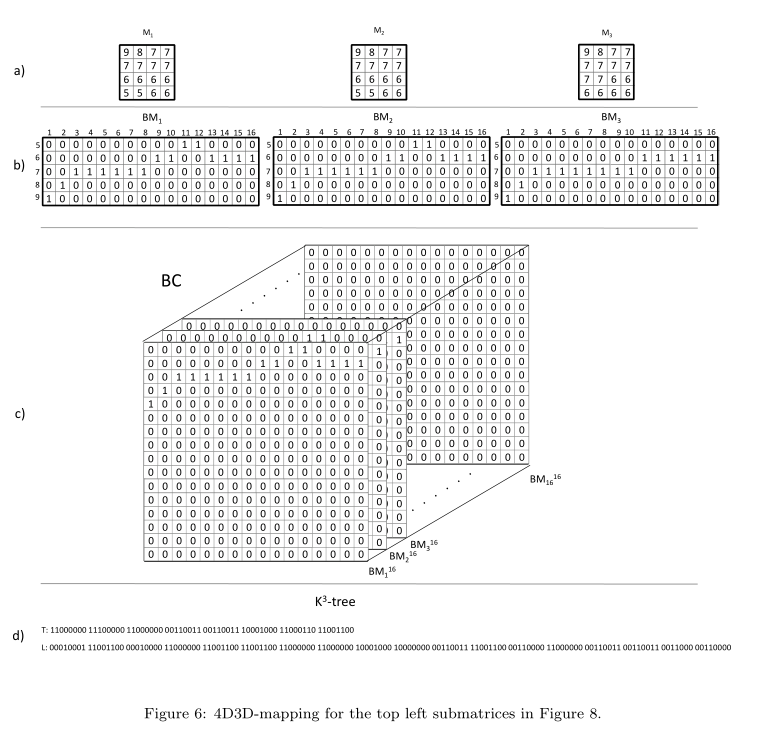
\includegraphics[width=0.8\textwidth]{../images/4d3d.png}

\end{itemize}

\section*{Problem definition}
\begin{itemize}
  \item Tenemos una secuencia de matrices raster para distintos instantes de
    tiempo $\tau$. Asumimos que cada celda de los raster almacena un entero.
\end{itemize}

\subsection*{Querys}
Vamos a lidiar con los siguientes tipos de querys:
\begin{itemize}
  \item $access(r,c,t)$: entrega el valor de la celda $(r,c)$ en el instante $t$.
  \item $windowQuery(r_1, r_2, c_1, c_2, t_1, t_2)$: Entrega todos los valores
    en el cuboide rectangular de esquinas $(r_1, c_1)$ y $(r_2, c_2)$ en un
    intervalo de tiempo $[t_1, t_2]$.
  \item $rangeQuery(r_1, r_2, c_1, c_2, t_1, t_2, rMin, rMax)$:
    Entrega todos los valores en el cuboide rectangular de esquinas $(r_1, c_1)$
    y $(r_2, c_2)$ en un intervalo de tiempo $[t_1, t_2]$ y entre un rango de
    valores $[rMin, rMax]$.\\
    Esta consulta es la más general y engloba al resto, las cuales corresponden a
    casos particulares de esta.
\end{itemize}

\subsection*{Q-cols \& Q-rows}
\begin{itemize}
  \item Dada una matriz de $n \times n$, la dividimos en $k$ grupos.
  \item Habrán $\frac{n}{k}$ $q-cols \text{ y } q-rows$.
  \item Dada una q-row, q-row$_i$ y la fila original $r \text{ | } r \in
    \{0,\ldots,n-1\}$, definimos $relative\_row(\text{q-row}_i,r)$ de la
    siguiente forma:
    \begin{itemize}
      \item Si $r \in q-row_i$, retorna la posición relativa de $r$ dentro de
        q-row$_i$.
      \item Si $r$ está en una q-row anterior a q-row$_i$, retorna 0.
      \item Si $r$ está en una q-row posterior a q-row$_i$, retorna
        $\frac{n}{k}-1$.
    \end{itemize}
  \item La función $relative\_col(q-col_i, r)$ funciona de manera análoga.
    \begin{figure}[h]
      \centering
      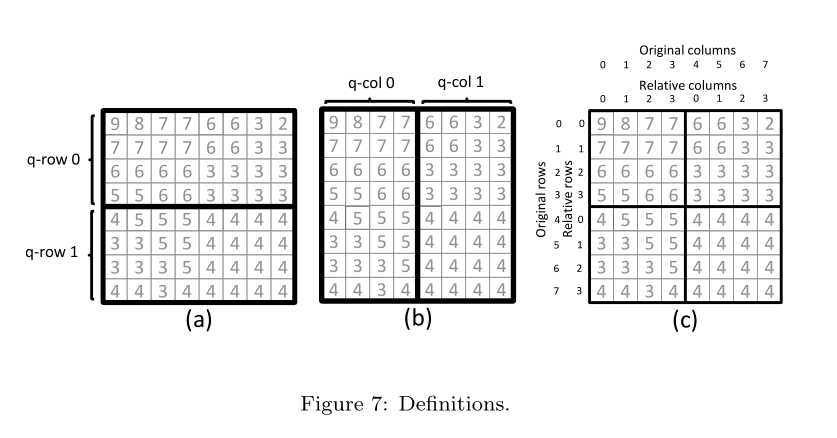
\includegraphics[width=0.8\textwidth]{../images/qrow.png}
    \end{figure}

\end{itemize}

\section*{T-k$^2$raster}

\begin{itemize}
  \item Basado en el $k^2raster$ y una combinación de \emph{snapshots} y
    \emph{logs}.
  \item La idea es usar muestreo a intervalos regulares de tamaño $t_\delta$.
  \item Snapshots: Representación de matrices raster en ciertos instantes de
    tiempo.
  \item Logs: Instantes de tiempo restantes con codificación diferencial.
  \item Más formalmente, matrices raster correspondientes a instantes de tiempo
    muestreados,\\
    $M_s \text{,  }s = i + 1 \cdot t_\delta$,  $i \in [0, (\tau - 1) / t_\delta]$
    , son completamente representados con un $k^2raster$, y nos referimos a ellos
    como \emph{snapshots}.
  \item Las $t_\delta - 1$ matrices raster $M_t$, $t \in [s+1, s+t_\delta-1]$
    que siguen  un snapshot $M_s$, son codificados usando a $M_s$ como
    referencia. Para hacer esto creamos un $k^2raster'$ modifcado para
    representar $M_t$.
\end{itemize}
    \subsection*{$k^2 $raster}
\begin{itemize}
  \item El $k^2raster'$ es similar al $k^2raster$, pero en cada paso del
    proceso de construcción, los valores de los quadboxes son codificados como
    diferencias con respecto a los quadboxes correspondientes en $M_s$, en vez
    de diferencias con respecto al nodo padre, como se hacía en el $k^2raster$
    regular.
  \item En el $k^2raster'$ también codificamos los valores máximos y mínimos
    de los nodos del árbol conceptual de $M_t$ como diferencias a los valores
    correspondientes a los nodos del \emph{snapshots}.
  \item En adición, si un quadbox en $M_t$ es idéntico, o todos sus valores se
    diferencian en un único valor $\alpha$ al mismo quadbox en $M_s$, dejamos
    de dividir recursivamente y guardamos una referencia a ese quadbox de
    $M_s$ y a la diferencia $\alpha$.
  \item Guardar esa referencia es barato, ya que solo tenemos que marcar en el
    árbol conceptual de $M_t$, que para el sub-árbol con raíz en un nodo dado $p$
    , tiene la misma estructura que el del árbol de $M_s$.
  \item Para este propósito, el $k^2tree'$ incluye además otro bitmap $eqB$,
    alineados a los ceros en $T$.
  \item Si $T[i] = 0$ (nodo sin hijos), entonces  $eqB[rank_0(T,i)] \gets 1$ y
    $Lmax[i] \gets \alpha$.
  \item Además, si $T[i] = 0 $, seteamos $eqB[rank_0(T,i)] \gets 0$ y
    $Lmax[i] \gets \beta$ (donde $\beta$ es la diferencia entre los valores
    máximos de ambos quadboxes, como los valores del instante de tiempo es
    almacenado como esa diferencia) para manejar el caso donde el quadbox
    correspondiente de $M_t$ tiene todas las celdas con el mismo valor (como en
    un $k^2raster$ regular).
  \item La construcción del $k^2raster'$ para la matriz $M_t$ relacionada al
    snapshot $M_s$ se puede resumir como, Sea $T_t$ un bitmap, $Lmax_t$ y
    $Lmin_t$ arreglos, todos ellos cumpliendo la misma función que en un
    $k^2raster$ normal.
  \item Partiendo de la matriz completa $M_t$ seguimos un proceso recursivo.
    Consideramos $q_t_j$ el quadbox de $M_t$ que está siendo procesado, y
    $q_s_j$ el quadbox relacionado en $M_s$.
  \item $maxval_t$ y $minval_t$; valores max y min de $q_t_j$.
  \item $maxval_s$ y $minval_s$ ; valores max y min de $q_s_j$.
  \item $z_t_j$ ; posición en el bitmap $T_t$ correspondiente a $q_t_j$.
  \item Si $q_t_j$ es un quadbox de $1 \times 1$, $Lmax_t[z_t_j] \gets
    (maxval_t - maxval_s)$ y la recursión se detiene.
  \item Como el $k^2raster$ lidia con valores positivos y negativos, se aplica
    \emph{folklore zigzag} para mapear negativos a positivos.
  \item Si $maxval_t == minval_s$; el proceso recursivo para. Seteamos $T_t
    [z_t_j] \gets 0$, $eqB[rank_0(T_t,z_t_j)] \gets 0$ y $Lmax_t[z_t_j] \gets
    (maxval_t - maxval_s)$.
\item Si $q_t_j$ y $q_t_s$ difieren por completo en $\alpha$,
				$T_t[z_t_j] \gets 0$, $eqB[rank_0(T_t,z_t_j)] \gets 1$ y
			$Lmax[z_t_j] \gets \alpha$.
        \centering
        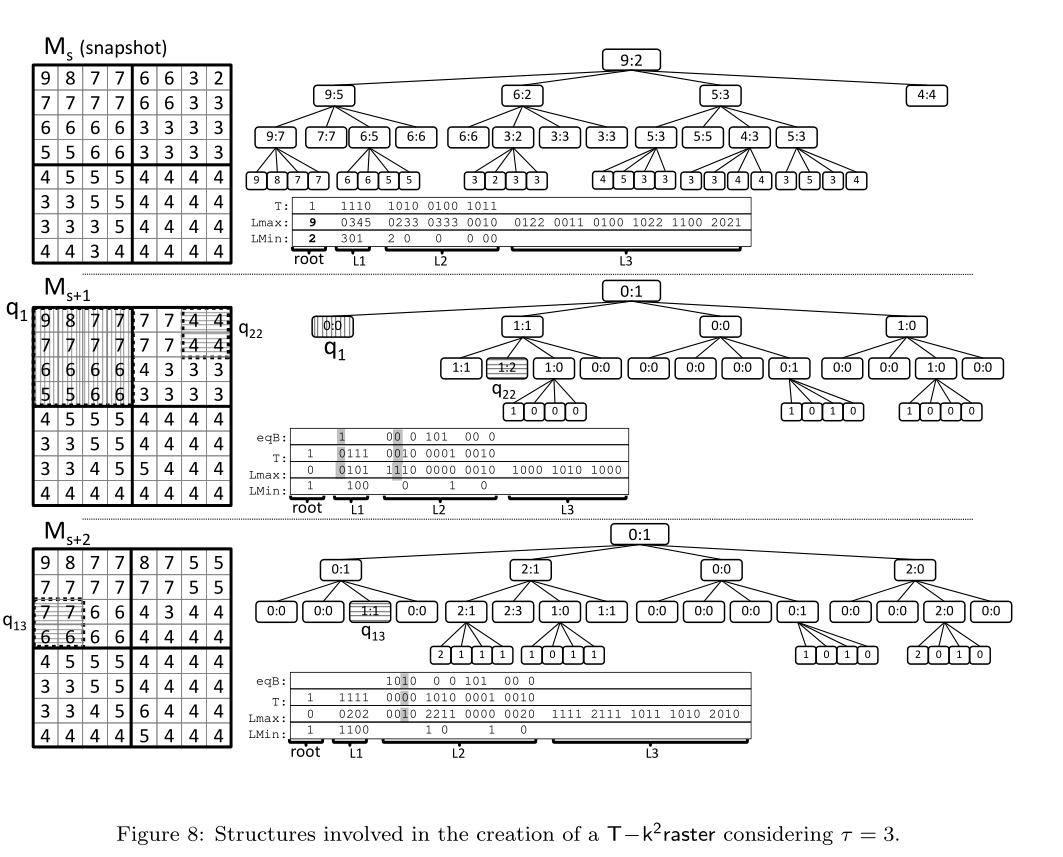
\includegraphics[width=0.8\textwidth]{../images/k2tin.png}
\item Con todo lo visto anteriormente ya podemos comprender el algoritmo de
  contrucción del $k^2$raster'.

    \centering
    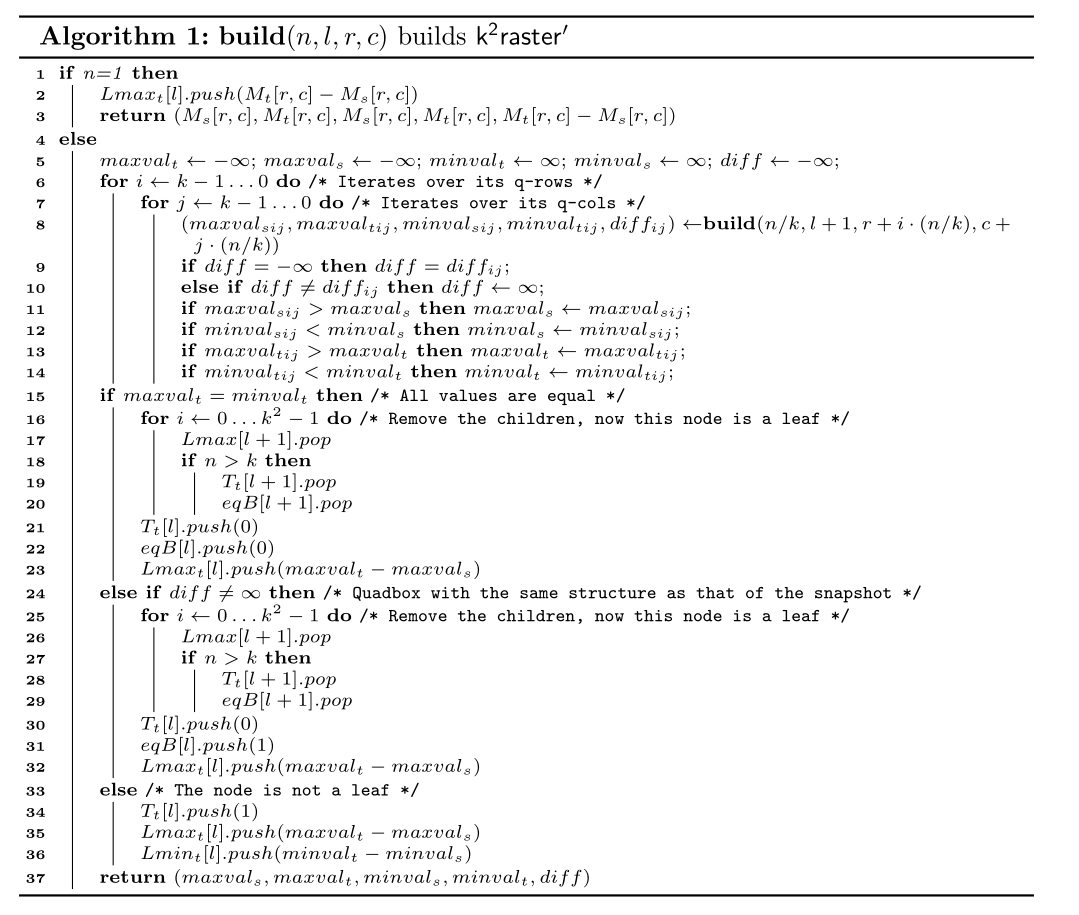
\includegraphics[width=0.8\textwidth]{../images/al1.png}

\end{itemize}

\subsection*{Querying}
\subsubsection*{Obtener el valor de una celda en un instante de tiempo}
\begin{itemize}
  \item Dos Casos:
    \item Si estamos haciendo la consulta sobre un snapshot, usamos el algoritmo
      para obtener el valor de una celda de un $k^2$ raster normal.
    \item En caso contrario, utilizamos un recorrido top-down sincronizado
      de los árboles representando a $M_t$ y al snapshot previo más cercano.
\end{itemize}
\begin{figure}[h]
  \centering
  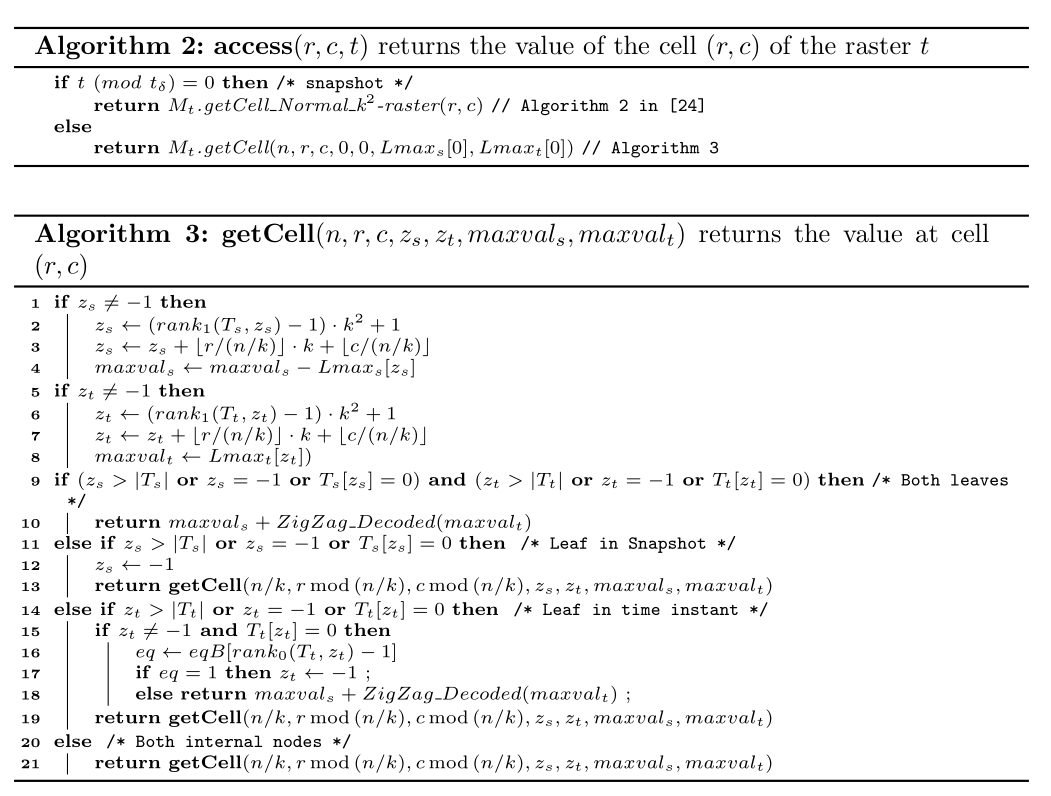
\includegraphics[width=0.8\textwidth]{../images/al2.png}
\end{figure}

\clearpage
\subsection*{Obtener un rango espacial}

\begin{itemize}
  \item Al igual que la query anterior tenemos 2 casos:
    \item Si estamos haciendo la consulta en un snapshots, utilizamos el
      algoritmo de un $k^2$raster para resolver esta operación.
    \item En caso contrario, debemos hacer un recorrido top-down sincronizado
      de los árboles representando a $M_t$ y al snapshot previo más cercano.
      La diferencia con la query anterior es que el recorrido puede requerir
      varias ramas de ambos árboles, ya que la región consultada se puede
      superponer a los quadboxes correspondientes a varios nodos del árbol.
\end{itemize}
\begin{figure}[h]
  \centering
  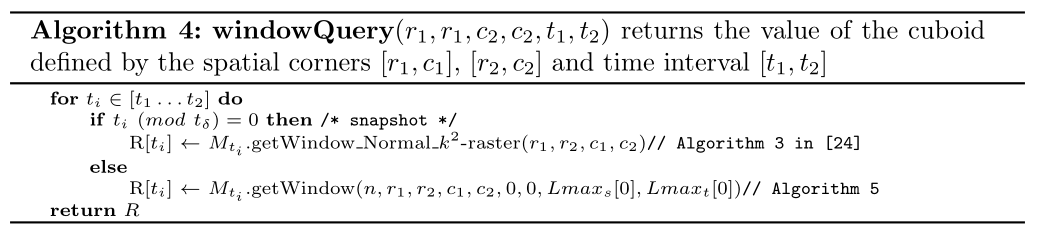
\includegraphics[width=0.8\textwidth]{../images/al4.png}
  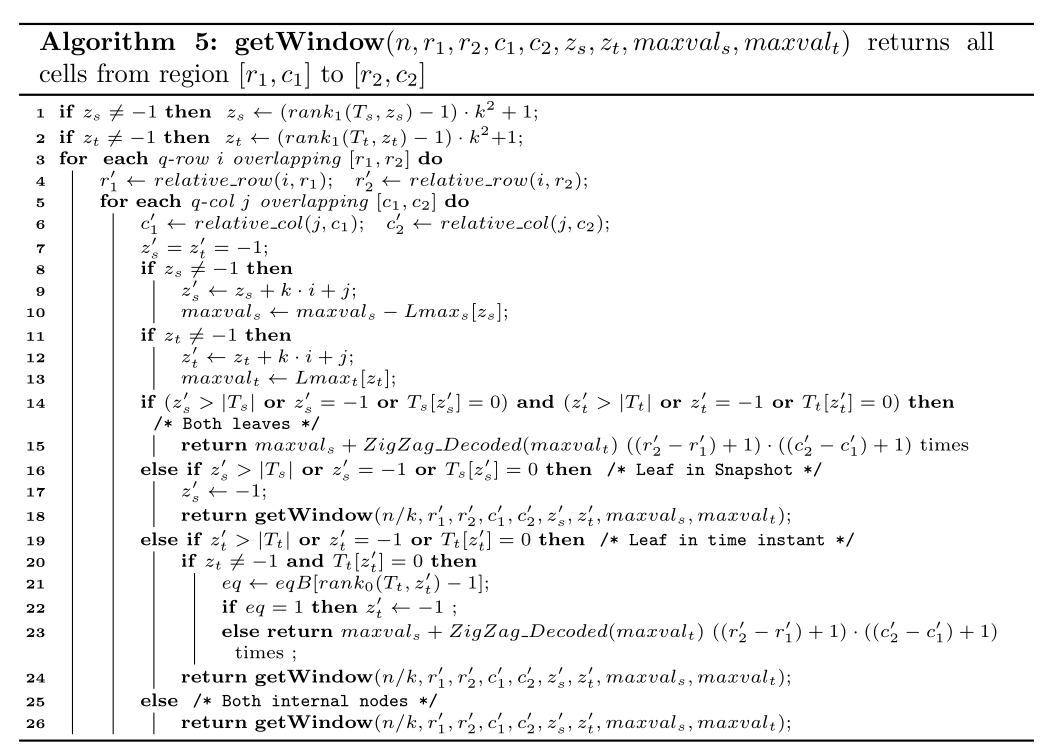
\includegraphics[width=0.8\textwidth]{../images/al5.png}
\end{figure}

\clearpage
\subsection*{Obtener celdas dentro de un rango de valores}
\begin{figure}[h]
  \centering
  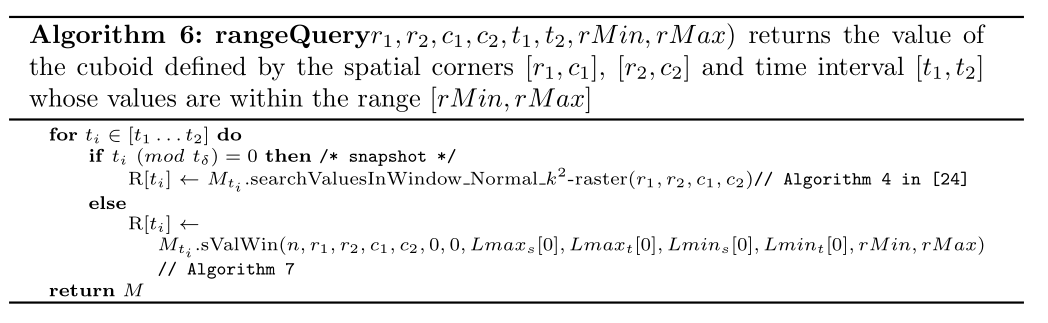
\includegraphics[width=0.8\textwidth]{../images/al6.png}
  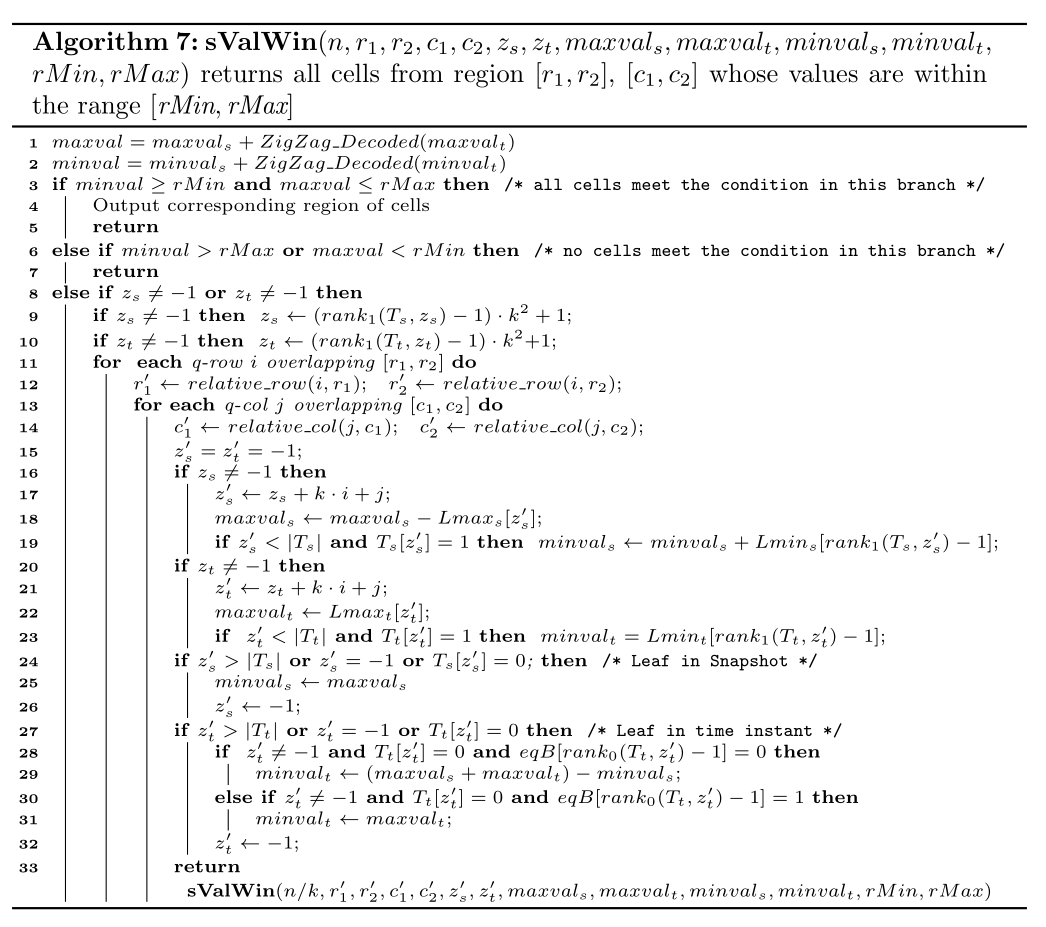
\includegraphics[width=0.8\textwidth]{../images/al7.png}
\end{figure}

\end{document}

